\chapter{Uncertainty}
Working on the previous circuit showd in \ref{fig:transmission_line_qubit}, we now consider a variation of the capacitance $C_g\,=\,50$fF\,$\pm5$\% over 100 samples using a Monte Carlo method.
\section{Analysis of the simulation}
Focussing on the case of $Lr1=9.006n$H ($f_r=7.5Ghz$), the resonance frequency of the resonator coupled with the system without any variation of $C_g$ is $f_r=3.29Ghz$, while inserting uncertainty 
this nominal value is spreaded over a range of $\approx120Mhz$ (see \ref{fig:spread_zoom}). This spread is far larger than the shift in the resonance frequency due to the qubit's state, which is of the order of $\approx10MHz$. This points out the importance of the reliabilty of the components and the minimization of the stochastic noise in the system.\\ 
\begin{figure}[H]
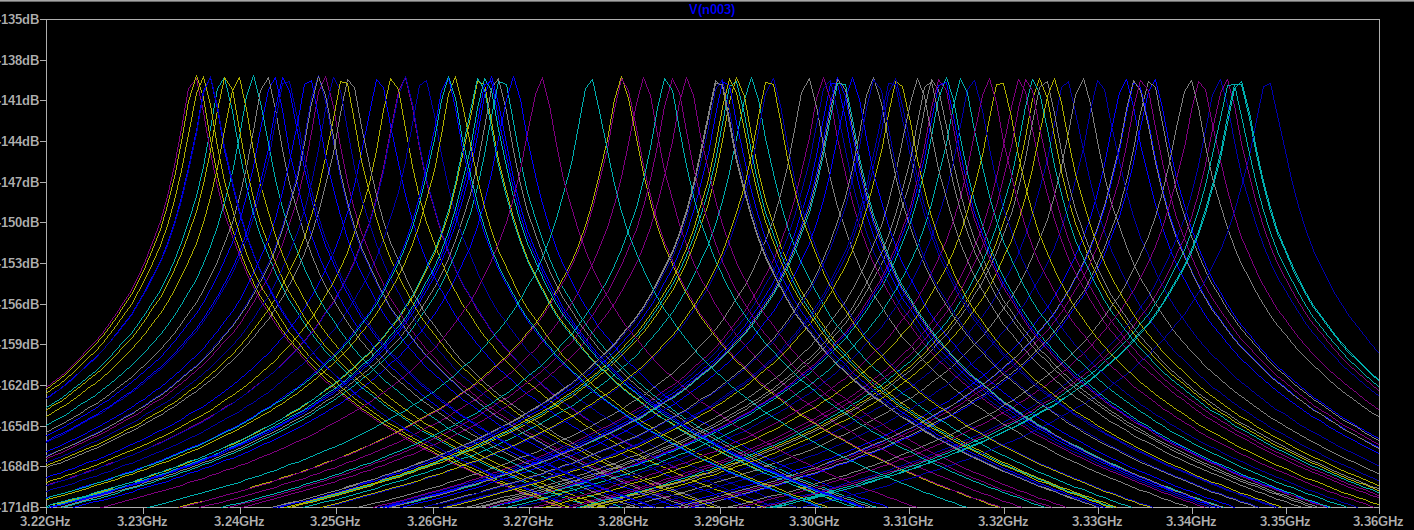
\includegraphics[width=1\linewidth]{exercise 8/spread_zoom.png}
\caption{Spread of $f_r$ }
\label{fig:spread_zoom}
\end{figure}
To mitigate the impact of the uncertainty in $C_g$, one can lower its nominal value, which will result in a less sensitive frequency shift ($\approx60MHz$) due to its variation as shown in \ref{fig:spread_lowc}.\\
However, this leads also to a smaller quality factor $Q$ of the resonator and so to a less sharp resonance peak, representing a higher loss-rate $k = \frac{f_r*2\pi}{Q}$. This introduce a trade-off between the robustness of the system to the uncertainty and the quality of the resonator.
\begin{figure}[H]
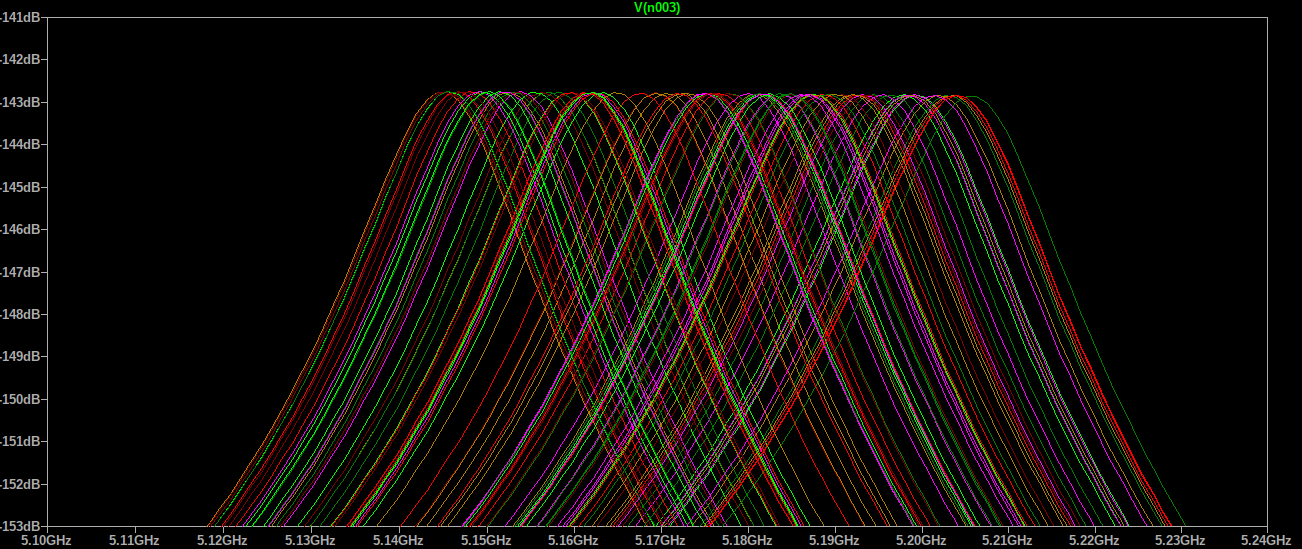
\includegraphics[width=1\linewidth]{exercise 8/spread_lowc.png}
\caption{Spread of $f_r$ with $C_g=7$fF}
\label{fig:spread_lowc}
\end{figure}